%!TEX root = ../main.tex
\part{Fundamentals of Quasi-Monte Carlo Methods}
\label{part1}

\chapter{Monte Carlo and Quasi-Monte Carlo Integration}
\label{chapter1}

% ------------------------------------------------------------------------------
% ------------------------------------------------------------------------------
\section{Motivation and Problem Setting}
% ------------------------------------------------------------------------------
% ------------------------------------------------------------------------------
The numerical evaluation of high-dimensional integrals is a fundamental task in
modern applied mathematics and scientific computing. Applications range from
Bayesian inference and financial mathematics to machine learning and
computational physics. In particular, contemporary domains such as deep neural
network training and medical imaging often require the estimation of integrals
of the form

\begin{equation}
    \label{eq:integration_problem}
    I = \int_{[0,1]^s} f(x)\,dx\,,
\end{equation}

where $s$ denotes the dimensionality of the problem and $f$ is a function that
may be expensive or impractical to evaluate analytically.

One of the most widely used approaches to compute such integrals is the
classical \ac{mc} method, which estimates the expectation based on averages over
randomly sampled points. The primary appeal of \ac{mc} integration lies in its
dimension-independent convergence rate and minimal assumptions on the integrand.
However, its asymptotic error rate of $\mathcal{O}(N^{-1/2})$ limits its
efficiency -- especially when high precision is required or function evaluations
are computationally expensive.

\ac{qmc} methods offer an alternative paradigm: instead of random samples, they employ deterministic sequences -- so-called low-discrepancy sequences—that aim to fill the integration domain more uniformly. This structured sampling allows for faster convergence under certain smoothness conditions and forms the basis for many state-of-the-art techniques in high-dimensional numerical integration.

The goal of this part is to develop a rigorous mathematical foundation for
\ac{qmc} methods and to understand how they improve upon classical Monte Carlo
integration. The key concepts introduced here -- particularly discrepancy theory
and low-discrepancy sequences -- serve as theoretical tools that will be
revisited in later parts of this thesis.
Chapter~\ref{chapter2} will delve into the
measurement of uniformity via star discrepancy and provide concrete
constructions of low-discrepancy sequences such as Sobol and Halton, which are
central to the numerical methods applied in Part~\ref{part2} and
Part~\ref{part3}, dedicated to neural network training and CT-based photon
transport simulation.


% ------------------------------------------------------------------------------
\subsection{High-Dimensional Integration in Applications}
% ------------------------------------------------------------------------------
High-dimensional integration problems arise naturally in a wide range of
scientific and engineering disciplines. Whenever expectations with respect to
multivariate distributions must be computed numerically, they are typically
formulated as integrals over the $s$-dimensional unit cube -- such as the
integral in Equation~\eqref{eq:integration_problem}.

Prominent examples include:
\begin{itemize}
    \item \textbf{Bayesian statistics}: Computing posterior expectations, marginal likelihoods, or predictive distributions.
    \item \textbf{Financial mathematics}: Pricing complex financial derivatives and evaluating risk measures under stochastic models.
    \item \textbf{Machine learning}: Estimating expectations in variational inference, training neural networks using randomized optimization techniques, or evaluating generalization bounds.
    \item \textbf{Medical imaging}: Simulating photon transport and estimating physical quantities based on noisy measurements, especially in \ac{ct} and magnetic resonance imaging (MRI).
\end{itemize}

In all these cases, the dimensionality $s$ can be moderate to very high --
sometimes even exceeding hundreds or thousands of variables. This introduces
significant challenges for numerical integration methods, which must balance
accuracy, computational cost, and robustness with respect to the structure of
the integrand.

The remainder of this chapter explores how \ac{mc} and \ac{qmc} methods address
these challenges. Before doing so, we briefly review the Monte Carlo method and
its fundamental convergence properties in the next section.


% ------------------------------------------------------------------------------
\subsection{Monte Carlo Integration: Principle and Convergence}
% ------------------------------------------------------------------------------
The classical \ac{mc} method is a probabilistic approach to numerical
integration that relies on random sampling. It is particularly suited for
high-dimensional settings, as its convergence rate does not deteriorate with
increasing dimension.

\begin{definition}[Monte Carlo Estimator] \ \\
Let $f \in L^2([0,1]^s)$ and let $X_0, \dots, X_{N-1} \sim
\mathcal{U}([0,1]^s)$ be independent and identically distributed random samples.
The Monte Carlo estimator of the integral \( I \) is given by
\begin{equation}
    I_N^{\mathrm{MC}} := \frac{1}{N} \sum_{n=0}^{N-1} f(X_n)\,.
\end{equation}
\end{definition}


This estimator is unbiased and converges almost surely to the true integral as $N \to \infty$, as established by the Strong Law of Large Numbers:

\begin{theorem}[Strong Law of Large Numbers] \ \\
Let $f \in L^2([0,1]^s)$. Then
\begin{equation}
\mathbb{P}\left[ \lim_{N \to \infty} Q_{N}(f) = \int_{[0,1]^s} f(x)\, dx \right] = 1.
\end{equation}
\end{theorem}

Beyond this almost sure convergence, the expected integration error of the Monte
Carlo estimator can be quantified using the root-mean-square error:

\begin{theorem}[Monte Carlo Convergence Rate, {\cite[Satz~1.2]{pillichshammer2010zahlentheoretische}}] \ \\
\label{thm:mc-convergence-rate}
Let $f \in L^2([0,1]^s)$. Then
\begin{equation}
    \mathbb{E}\left[ \left| Q_{N}(f) - I \right| \right] \leq \frac{\sigma[f]}{\sqrt{N}},
\end{equation}
where $\sigma[f] := \sqrt{\mathrm{Var}[f]}$.
\end{theorem}

\begin{proof}[Sketch of Proof]
Using independence and linearity of expectation, the variance of $Q_N(f)$ is
\begin{equation}
    \mathrm{Var}[Q_N(f)] = \frac{\mathrm{Var}[f]}{N}.
\end{equation}
Applying Jensen's inequality yields the stated bound on the expected absolute error.
\end{proof}

\begin{remark}
The convergence rate $\mathcal{O}(N^{-1/2})$ is independent of the integration
dimension $s$, which is a key advantage of the Monte Carlo method. In contrast,
classical grid-based methods often suffer from the curse of dimensionality,
where the number of required samples grows exponentially with $s$.
\end{remark}

\begin{example}
Let $f \in C^1([0,1]^s)$ be a Lipschitz-continuous function. A uniform grid with
$N = m^s$ points has a worst-case error of $\mathcal{O}(N^{-1/s})$. In high
dimensions, this becomes prohibitively inefficient, while MC integration retains
the dimension-agnostic rate $\mathcal{O}(N^{-1/2})$. \cite[Section
1.1]{leobacher2014introduction}
\end{example}

Despite its robustness and simplicity, MC integration has several well-known limitations:
\begin{itemize}
    \item The convergence rate is relatively slow, especially for smooth integrands.
    \item Error bounds are probabilistic rather than deterministic.
    \item The method does not exploit structural properties of the integrand, such as smoothness or sparsity.
\end{itemize}

These limitations motivate the development of quasi-Monte Carlo methods, which
will be introduced in the next section.


% ------------------------------------------------------------------------------
% ------------------------------------------------------------------------------
\section{Quasi-Monte Carlo Methods}
% ------------------------------------------------------------------------------
% ------------------------------------------------------------------------------

% ------------------------------------------------------------------------------
\subsection{Deterministic Sampling and Intuition}
% ------------------------------------------------------------------------------

Classical \ac{mc} methods approximate integrals over the unit cube $[0,1]^s$
using randomly sampled points. In contrast, \ac{qmc} methods replace
stochasticity with a deterministic strategy, aiming to cover the integration
domain in a more uniform and structured way.

\begin{definition}[Quasi-Monte Carlo Estimator] \ \\
Let $f \colon [0,1]^s \to \mathbb{R}$ be a measurable function and let
$\{\boldsymbol{x}_n\}_{n=1}^{N} \subset [0,1]^s$ be a deterministic point set.
Then the \emph{quasi-Monte Carlo estimator} for the integral
\begin{equation*}
    I(f) = \int_{[0,1]^s} f(\boldsymbol{x}) \, d\boldsymbol{x}
\end{equation*}
is defined as
\begin{equation}
I_N^{\mathrm{QMC}}(f) := \frac{1}{N} \sum_{n=1}^{N} f(\boldsymbol{x}_n).
\end{equation}
\end{definition}

Unlike in the Monte Carlo setting, these points are not drawn from a probability
distribution, but are generated deterministically — typically by rules that aim
to avoid clustering and oversampling.

Figure~\ref{fig:mc-vs-qmc} illustrates this contrast by comparing $300$ randomly
sampled points to $300$ \ac{qmc} points from the Sobol' sequence in two
dimensions. The quasi-Monte Carlo points distribute more evenly, avoiding both
gaps and clusters.

\begin{figure}[H]
  \centering
  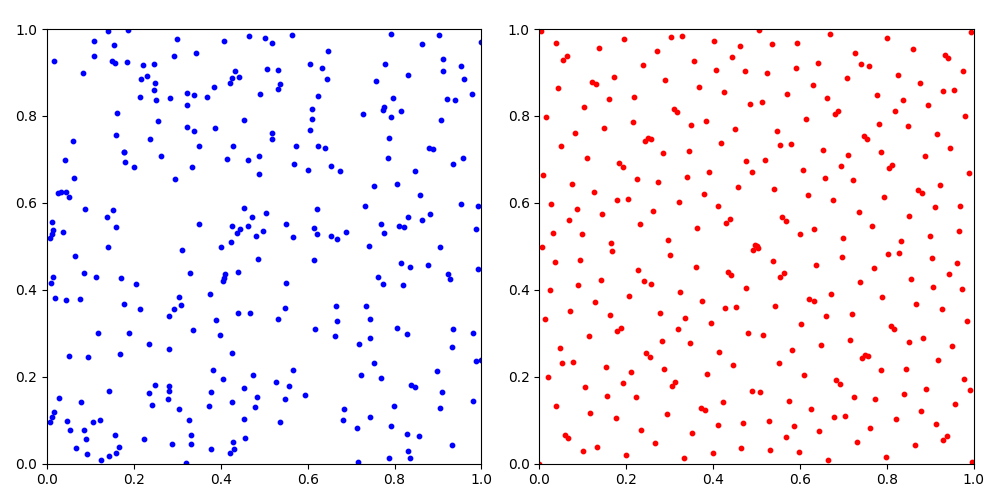
\includegraphics[width=0.8\textwidth]{Figures/mc_vs_qmc.png}
  \caption{Comparison of $300$ sample points in $[0,1]^2$ using (left) standard 
  Monte Carlo and (right) a Sobol' sequence. \ac{qmc} points avoid clustering and 
  fill the domain more evenly.}
  \label{fig:mc-vs-qmc}
\end{figure}

A natural alternative to \ac{mc} sampling is the use of regular tensor-product
grids. However, these grids suffer from the \emph{curse of dimensionality}:
placing $m$ points per dimension leads to a total of $N = m^s$ points, which
becomes infeasible even for moderate $s$. Furthermore, grids are not easily
extensible -- adding new points requires global recomputation and destroys
nesting.

By contrast, many \ac{qmc} sequences, such as Sobol' and Halton (introduced in
Chapter~\ref{chapter2}), are designed to be \emph{incremental}: each new point
can be added without changing the existing ones. This makes \ac{qmc}
particularly suitable for adaptive and anytime algorithms. However, not all
\ac{qmc} constructions share this feature such as lattice rules and some
optimized designs are fixed-size by nature.

\ac{qmc} methods thus offer the best of both worlds: they combine the
space-filling structure of grids with the flexibility and scalability of
sampling methods. Low-discrepancy sequences fill the space more evenly than
random points while avoiding the redundancy of regular grids. This often leads
to significantly lower integration errors, especially for smooth functions or
problems with low effective dimension.

This shift from probabilistic to deterministic sampling also changes the way we
analyze error: instead of using statistical bounds, we rely on \emph{discrepancy
measures}, which quantify the uniformity of the point set. These concepts, along
with the notion of function variation, will be introduced in the following
sections.

\begin{remark}
\ac{qmc} estimators retain the same algebraic structure as their \ac{mc}
counterparts, but their convergence behavior is governed by entirely different
theoretical tools -- namely discrepancy theory and function variation.
\end{remark}


% ------------------------------------------------------------------------------
\subsection{Monte Carlo vs. Quasi-Monte Carlo: A First Comparison}
\label{subsec:mc-vs-qmc}
% ------------------------------------------------------------------------------

\ac{mc} and \ac{qmc} methods share the same high-level goal: estimating an
integral by averaging function evaluations at selected sample points. The
difference lies in the sampling strategy -- stochastic versus deterministic --
and the consequences this has for accuracy, convergence and theoretical
guarantees.

Table~\ref{tab:mc-vs-qmc} summarizes key conceptual distinctions between the two paradigms.

\begin{table}[H]
\centering
\resizebox{0.95\textwidth}{!}{
\renewcommand{\arraystretch}{1.4}
\begin{tabular}{l|c|c}
\textbf{Aspect} & \textbf{Monte Carlo (MC)} & \textbf{Quasi-Monte Carlo (QMC)} \\
\hline
Sampling & Independent random points & Deterministic low-discrepancy points \\
Error bounds & Probabilistic (in expectation) & Deterministic (worst-case) \\
Regularity assumptions on $f$ & Square integrability ($L^2$) & Bounded variation (HK) \\
Theoretical convergence & $\mathcal{O}(N^{-1/2})$ & Up to $\mathcal{O}(N^{-1})$ (heuristic) \\
Point extensibility & Trivial & Often supported (e.g., Sobol) \\
Robustness to noise & High & Low \\
\end{tabular}}
\caption{Conceptual comparison of Monte Carlo and quasi-Monte Carlo integration methods.}
\label{tab:mc-vs-qmc}
\end{table}

While \ac{mc} estimators are unbiased and robust even under minimal assumptions,
their convergence is slow and does not improve when the integrand is smooth.
\ac{qmc} methods, on the other hand, exploit structure in the integrand -- such
as smoothness or low effective dimension -- and can yield significantly lower
integration errors.

However, \ac{qmc} methods lack probabilistic guarantees and depend more strongly
on the careful construction of the point set. Their performance can degrade if
the integrand exhibits high variability along many input dimensions or if the
chosen sequence is not well matched to the function.

The next subsection discusses the convergence rates of both methods in more
detail and highlights the interplay between dimensionality and integration
error.


% ------------------------------------------------------------------------------
\subsection{Convergence Rates and the Curse of Dimensionality}
\label{subsec:convergence-vs-dimension}
% ------------------------------------------------------------------------------

A major appeal of the Monte Carlo method is its dimension-agnostic convergence
behavior from Theorem~\ref{thm:mc-convergence-rate}. Under the assumption that
$f \in L^2([0,1]^s)$, the root-mean-square error of the MC estimator satisfies

\begin{equation}
    \mathbb{E}[ | I_N^{\mathrm{MC}} - I |] = \mathcal{O}(N^{-1/2}),
\end{equation}

regardless of the dimension $s$. This makes \ac{mc} a go-to method for very
high-dimensional problems, even when no structure in the integrand is known or
exploitable.

\ac{qmc} methods, while lacking this universality, offer a fundamentally
different convergence profile. For sufficiently regular integrands
(specifically, those of bounded variation in the sense of Hardy and Krause), the
integration error of \ac{qmc} estimators is bounded by

\begin{equation}
    | I_N^{\mathrm{QMC}} - I | \leq D_N^* \cdot V_{\mathrm{HK}}(f),
\end{equation}

where $D_N^*$ is the star discrepancy of the point set and $V_{\mathrm{HK}}(f)$
is the Hardy--Krause variation of the integrand (both formalized later in
\textcolor{blue}{\textbf{TODO}}). For well-constructed low-discrepancy
sequences, it is known that

\begin{equation}
    D_N^* = \mathcal{O}\left( \frac{(\log N)^s}{N} \right).
\end{equation}

This bound implies a near-linear convergence rate in $N$ -- much faster than
\ac{mc} -- but introduces a logarithmic dependence on the dimension $s$. As $s$
increases, the factor $(\log N)^s$ grows rapidly, leading to the curse of
dimensionality in worst-case \ac{qmc} analysis.

Fortunately, in many practical problems, the \emph{effective dimension} of the
integrand is much lower than its nominal input dimension. That is, most of the
function's variation is concentrated along a small number of directions. When
this is the case, QMC methods frequently outperform MC in practice, even in
problems with moderately high $s$.

\begin{example}
In deep learning applications, such as training neural networks, stochastic
gradients often lie near low-dimensional manifolds. Similarly, in CT-based
simulation models, the system's physical response depends more strongly on a few
dominant input parameters. These scenarios are highly favorable for QMC.
\end{example}

We will revisit the precise meaning of discrepancy and variation -- and how they
control the QMC error -- in Chapters~\ref{chapter2} and \ref{chapter3}.


% ------------------------------------------------------------------------------
\section{Uniformity Concepts}
\label{sec:uniformity-concepts}
% ------------------------------------------------------------------------------

The efficiency of \ac{qmc} methods hinges on how well the employed point sets
"fill" the integration domain $[0,1]^s$. This motivates the need for a precise
mathematical understanding of \emph{uniformity}. The present section introduces
two key concepts in this regard -- \emph{uniform distribution modulo one} and
\emph{equidistribution} -- and clarifies their relevance to numerical
integration.

% ------------------------------------------------------------------------------
\subsection{Uniform Distribution vs. Equidistribution}
% ------------------------------------------------------------------------------

While the terms \emph{uniform distribution} and \emph{equidistribution} are
sometimes used interchangeably in informal contexts, they carry distinct
meanings in the context of numerical integration. In quasi-Monte Carlo methods,
the notion of \emph{uniform distribution modulo one} provides a rigorous
criterion for how evenly a sequence covers the unit cube. This concept forms the
foundation for analyzing the convergence behavior of QMC estimators.

\begin{definition}[Uniform Distribution Modulo One] \ \\
Let $(\boldsymbol{x}_n)_{n \in \mathbb{N}_0} \subset [0,1]^s$ be a sequence of
sample points. The sequence is said to be \emph{uniformly distributed modulo
one} (u.d.\ mod~1) if, for every axis-aligned box $[\boldsymbol{a},
\boldsymbol{b}) \subset [0,1]^s$, the proportion of points falling into this box
converges to its Lebesgue measure:
\begin{equation*}
    \lim_{N \to \infty} \frac{1}{N} \sum_{n=0}^{N-1} \chi_{[\boldsymbol{a}, \boldsymbol{b})}(\boldsymbol{x}_n)
    = \lambda_s([\boldsymbol{a}, \boldsymbol{b})) \,,
\end{equation*}
where $\lambda_s$ denotes the $s$-dimensional Lebesgue measure and $\chi_A$ is
the indicator function of the set $A$.
\end{definition}

This definition emphasizes asymptotic spatial coverage: in the limit, every
subregion of the domain is sampled proportionally to its volume. Importantly,
this property is purely deterministic and does not rely on any probabilistic
assumptions — in contrast to Monte Carlo methods, which only guarantee
uniformity in expectation.

In contrast, when speaking of a random sample $\{X_1, \dots, X_N\} \subset [0,1]^s$ drawn i.i.d.\ from the uniform distribution, we refer to a probabilistic concept of uniformity: each point is independently drawn according to the uniform measure, but the empirical distribution may not be uniformly spread in finite samples. Thus, equidistribution refers to the ideal uniform coverage that we seek deterministically, while uniform random sampling only ensures this behavior in expectation or with high probability.

\begin{remark}
Uniform distribution modulo one is a necessary condition for the convergence of quasi-Monte Carlo estimators. If a point sequence is not u.d.\ mod 1, then there exists at least one Riemann-integrable function for which the sample average fails to converge to the integral.
\end{remark}

The following result, known as Weyl’s criterion, provides a necessary and sufficient condition for uniform distribution in terms of exponential sums.

\begin{theorem}[Weyl's Criterion] \ \\
A sequence $(\boldsymbol{x}_n)_{n \geq 0} \subset [0,1)^s$ is uniformly distributed modulo one if and only if, for all nonzero $\boldsymbol{h} \in \mathbb{Z}^s \setminus \{\boldsymbol{0}\}$, we have
\begin{equation*}
    \lim_{N \to \infty} \frac{1}{N} \sum_{n=0}^{N-1} \exp(2\pi i\, \boldsymbol{h} \cdot \boldsymbol{x}_n) = 0.
\end{equation*}
\end{theorem}

\begin{example}
Let $\alpha \in \mathbb{R}$ be irrational. Then the Kronecker sequence $(n \alpha \bmod 1)_{n \geq 0}$ is uniformly distributed in $[0,1]$. This is a consequence of Weyl’s criterion and illustrates the existence of simple, deterministic sequences with excellent uniformity properties.
\end{example}

% ------------------------------------------------------------------------------
\subsection{Why Uniformity Matters in Numerical Integration}
% ------------------------------------------------------------------------------

In \ac{qmc} integration, the objective is to approximate the integral defined in
Equation~\eqref{eq:integration_problem} by a finite average over a deterministic
point set $\{\boldsymbol{x}_0, \dots, \boldsymbol{x}_{N-1}\} \subset [0,1]^s$.
The accuracy of this approximation depends crucially on how uniformly the point
set samples the domain.

Unlike \ac{mc} methods, which rely on probabilistic guarantees and
variance-based error estimates, \ac{qmc} methods exploit deterministic
structure: the integration error is directly influenced by how well the point
set fills the domain. This insight gives rise to one of the most fundamental
theoretical tools in \ac{qmc} analysis: the \emph{Koksma--Hlawka inequality}.

\begin{remark}
The Koksma--Hlawka inequality bounds the integration error of a QMC estimator by
the product of two quantities: the \emph{star discrepancy} of the point set and
the \emph{variation} of the integrand in the sense of Hardy and Krause. In
short,
\begin{equation*}
    \left| \frac{1}{N} \sum_{n=0}^{N-1} f(\boldsymbol{x}_n) - I \right| 
    \leq D_N^*(\{\boldsymbol{x}_n\}) \cdot V_{\mathrm{HK}}(f).
\end{equation*}
A rigorous statement and detailed discussion of this inequality will follow in
Chapter~\ref{chapter3}.
\end{remark}

This inequality highlights why uniformity is essential: if the integrand has
bounded variation, then smaller discrepancy directly implies smaller integration
error. In this sense, discrepancy theory becomes a cornerstone of effective
\ac{qmc} integration.

\begin{remark}
The star discrepancy quantifies the maximal deviation between the empirical
distribution of the point set and the uniform distribution over $[0,1]^s$. It
vanishes asymptotically for uniformly distributed sequences and governs the
convergence behavior of \ac{qmc} estimators.
\end{remark}

The next chapter provides a formal introduction to discrepancy theory. We will
define extreme and star discrepancy, study their geometric interpretation, and
analyze the behavior of structured low-discrepancy sequences such as Halton and
Sobol'. These sequences, due to their uniform space-filling properties, play a
central role in modern high-dimensional numerical integration.
